\chapter{METHODOLOGY}
\section{Software Development Approach}
The project will follow an Agile software development methodology to ensure adaptability to evolving requirements and facilitate iterative progress. Scrum will be employed as the project management framework, promoting regular collaboration, timely milestone delivery, and continuous refinement of the Tourist Attraction Recommendation System.

\subsection{Project Planning}
A detailed project plan will be developed, outlining key milestones, deliverables, timelines, and resource allocation. Sprint planning sessions will define clear sprint goals, prioritize user stories, and estimate effort for each iteration. This structured approach will guide the team through the project and ensure alignment with the overall objectives.

\subsection{Requirements Gathering and Analysis}
User-centric requirements will be gathered through engaging potential tourists and travelers. This will involve understanding user preferences, travel behaviors, and specific needs for planning travel itineraries. Focus will be placed on tourist preferences, historical visit patterns, and geographic insights to develop a comprehensive understanding of what travelers seek in their trip planning. Data sources such as local tourist attraction databases, user feedback, and online platforms will be utilized to enrich the requirements. These insights will be used to define key functionalities and establish clear user stories and acceptance criteria, ensuring the system meets the specific needs of the travelers and provides a tailored recommendation experience.

\subsection{Iterative Development}
The project will be divided into iterations or sprints, typically lasting 2-4 weeks. Each sprint will focus on specific features, enhancements, or improvements identified in the product backlog. This iterative approach will ensure that the system evolves based on user feedback and real-world usage, adapting to changing user needs and improving the system with each cycle.

\subsection{Continuous Integration and Testing}
Continuous Integration (CI) practices will be implemented to enable frequent code updates and quick detection of integration issues. Rigorous testing, including both automated and manual testing, will be conducted throughout development to ensure system reliability, functionality, and high performance. Testing frameworks will be used for regression testing, performance testing, and usability testing to maintain the system’s quality and address issues proactively.

\subsection{Collaborative Feedback and Iteration}
Regular feedback sessions will be conducted to ensure the system meets user expectations. Usability testing, user acceptance testing, and the collection of feedback from test users will guide iterative refinements of the system. Emphasis will be placed on a culture of continuous improvement, allowing the system to evolve based on real-time data and user input, ensuring the most relevant and effective travel recommendations.

\subsection{Documentation and Reporting}
Comprehensive documentation will be maintained throughout the project, including detailed records of requirements specifications, user stories, design decisions, technical architecture, and testing results. This will ensure the project is well-documented for both current and future reference. Progress reports and sprint reviews will be provided to stakeholders, keeping them informed about milestones and achievements.Lessons learned and key decisions made during development will be documented to capture insights for future improvements and provide a clear understanding of the development process.

\begin{figure}[hbt!]
\centering
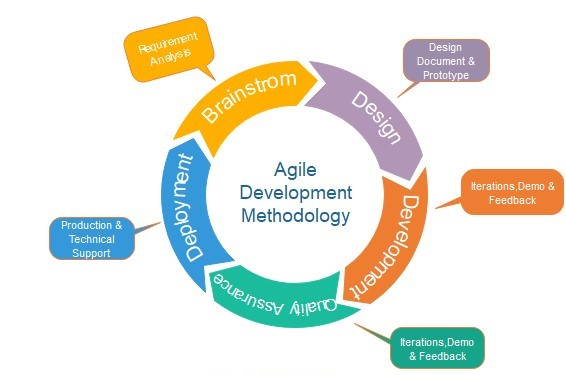
\includegraphics[width=0.75\textwidth]{./img/agile.jpg}
\caption{Agile Model for Software Development}
(Source: \href{https://www.javatpoint.com/software-engineering-agile-model}{Javapoint})
\end{figure}


\section{Block Diagram of Proposed System}
\begin{figure}[h]
\centering
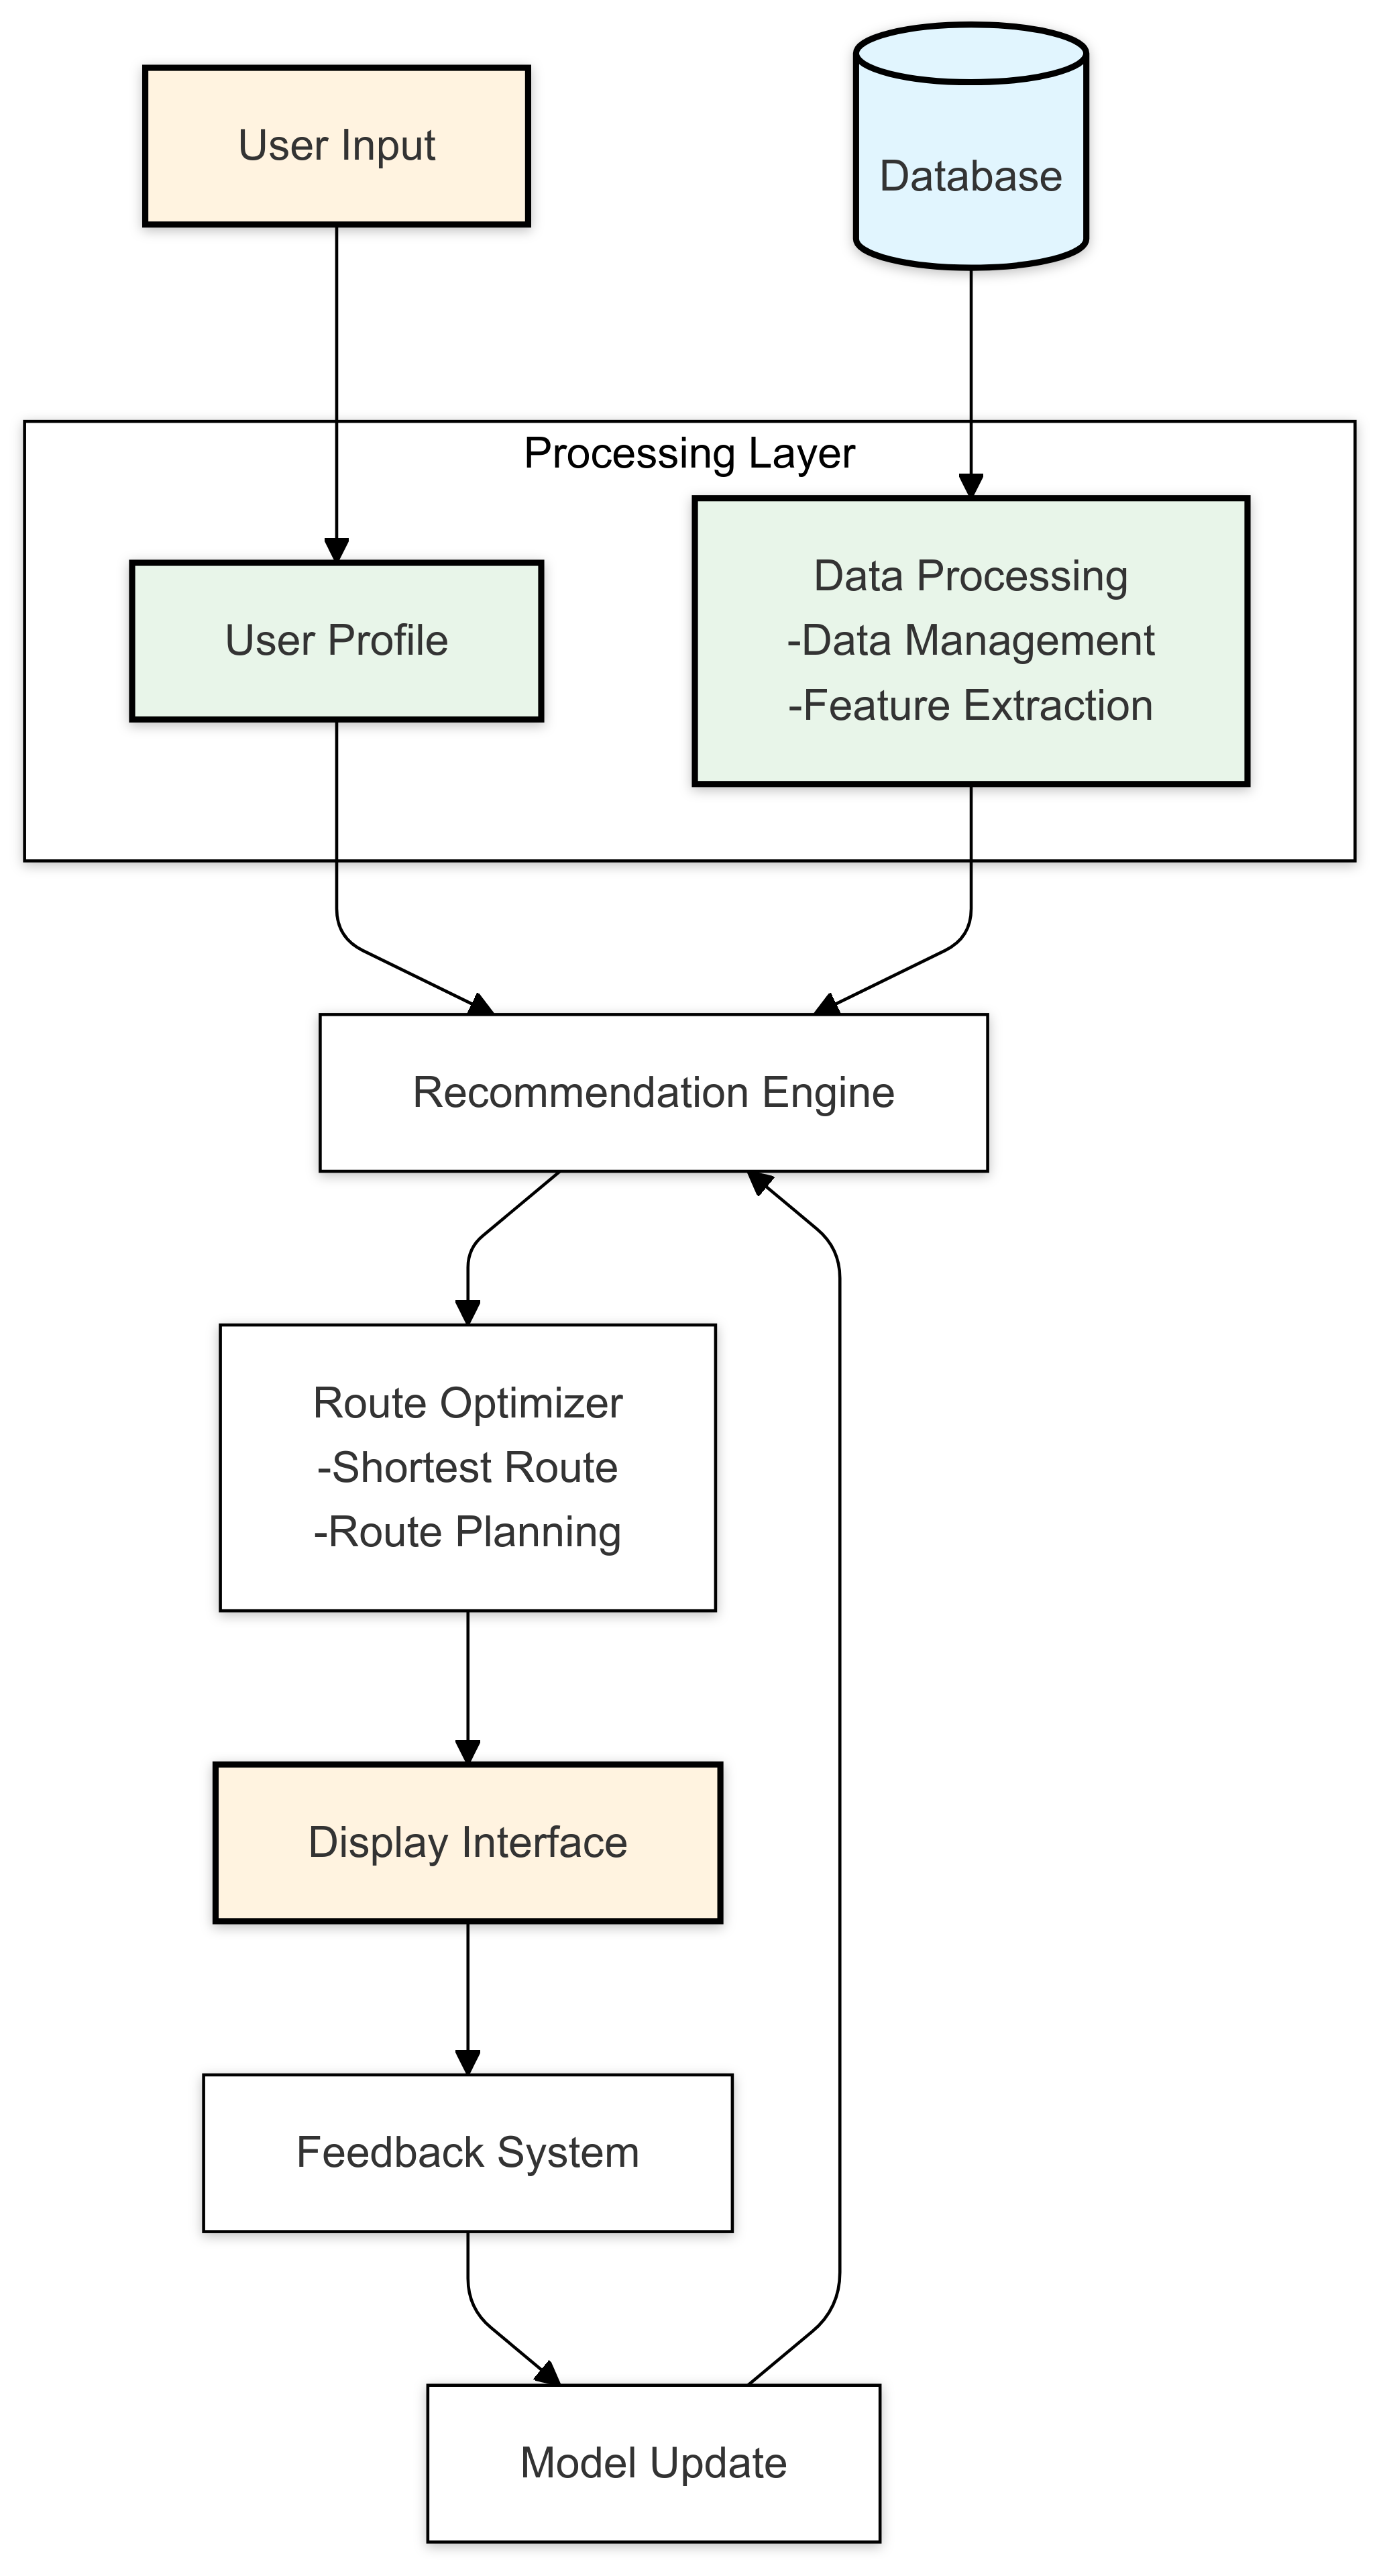
\includegraphics[width=0.5\textwidth]{./img/blockk1.png}
\caption{System Block Diagram}
\end{figure}

\section{Description of Working Flow of Proposed System}

\subsection{User Input (Preferences):}
This module captures user preferences, which are crucial for generating personalized recommendations. The user will be prompted to provide several inputs that will define their interests and constraints:
\begin{itemize}
    \item \textbf{Location}: Users specify their desired destination or a broader area of interest. This helps the system narrow down available tourist spots and tailor suggestions to the geographical region of the user’s choice.
    \item \textbf{Interests}: Users indicate their preferences regarding the types of activities or attractions they are interested in. These could include historical sites, nature reserves, museums, or cultural experiences, helping to focus the recommendations on specific types of attractions.
    %\item \textbf{Budget}: Users provide information about their financial limits for the trip. The system uses this to prioritize recommendations within the user’s specified price range, offering affordable or luxury options based on the user's needs.
    %\item \textbf{Time Constraints}: Users specify how much time they have for their visit, which allows the system to suggest locations that can be visited within the available time frame. It also helps to prioritize locations that align with the user’s schedule, such as locations with shorter visit times or those open during the user’s preferred hours.
\end{itemize}

\subsection{User Profile}
This module manages user profiles, which are essential for personalizing recommendations. The system tracks key user data, preferences, and past interactions to improve the accuracy of future suggestions:
\begin{itemize}
    \item \textbf{User Preferences}: The system stores detailed information on the user’s location preferences, activity interests, budget, and time constraints, allowing for personalized suggestions tailored to their needs.
    \item \textbf{Past Interactions}: The user’s previous interactions with the system, including previously recommended places, locations visited, and the user’s behavior while using the app, help refine future suggestions by identifying preferences and patterns.
    \item \textbf{Feedback History}: The system logs any user feedback about past recommendations, including ratings and comments on visited locations. This feedback is crucial for continually improving the recommendations and adjusting the system to the user’s evolving preferences.
\end{itemize}

\subsection{Attractions Database}
The attractions database is the foundation of the recommendation engine. It stores comprehensive details on tourist spots, including:
\begin{itemize}
    \item \textbf{Name}: The name of the tourist attraction.
    \item \textbf{Location}: The geographical location or address of the attraction.
    %\item \textbf{Description}: A short description of the attraction, providing users with insight into what they can expect.
    \item \textbf{Category/Type}: The type of attraction, such as a historical site, park, museum, cultural landmark, etc., which helps to filter recommendations based on the user’s interests.
    \item \textbf{Ratings and Reviews}: User-generated content providing ratings and comments on the attraction, which assists in evaluating its popularity and quality.
    %\item \textbf{Operating Hours}: Information on the opening and closing times, essential for users planning visits based on their schedules.
    %\item \textbf{Admission Fees}: Details on any entrance fees or tickets required to visit the attraction.
    %\item \textbf{Accessibility Information}: Information on how accessible the attraction is for people with disabilities, whether public transportation is available nearby, or if the location is family-friendly.
\end{itemize}

\subsection{Data Preprocessing}
Data preprocessing ensures that raw data is cleaned, structured, and ready for analysis by transforming it into a usable format for the recommendation system. This stage involves several tasks:
\begin{itemize}
    \item \textbf{Cleaning}: The raw data is cleaned by addressing missing values, removing duplicates, and correcting errors in the dataset.
    \item \textbf{Normalization and Standardization}: Numeric features, such as ratings or admission fees, are normalized or standardized to ensure consistency across different data sources.
    \item \textbf{Encoding Categorical Variables}: Categorical variables, such as attraction type or location, are converted into numerical values through encoding methods, making it easier for the recommendation model to process them.
    \item \textbf{Feature Engineering}: New features might be created or existing features transformed to improve the performance and accuracy of the recommendation system, such as calculating the average rating for a particular attraction or grouping attractions by category.
    \item \textbf{Dimensionality Reduction}: Techniques such as Principal Component Analysis (PCA) are applied to reduce the complexity of the dataset by identifying the most significant features, thus improving the speed and efficiency of the recommendation process.
\end{itemize}

\subsubsection{Data Management}
Effective data management is essential for ensuring that the recommendation engine operates smoothly. Key elements of data management include:
\begin{itemize}
    \item \textbf{Data Acquisition}: Gathering relevant and accurate data from reliable sources, such as tourist websites, user feedback, and official attraction listings.
    \item \textbf{Data Storage}: Storing the data in a secure, accessible manner, typically in a database or cloud storage system.
    \item \textbf{Data Security}: Implementing measures to protect sensitive user data, such as encryption and access controls, ensuring that privacy is maintained.
    \item \textbf{Data Governance}: Establishing rules and procedures for managing data quality, privacy, and consistency across the system.
    \item \textbf{Data Quality Management}: Ensuring the collected data is accurate, up-to-date, and relevant for generating useful recommendations.
\end{itemize}

\subsection{Recommendation Engine}
The recommendation engine is the heart of the proposed system. It generates personalized suggestions based on the user’s preferences and the data in the attractions database. The system uses a combination of collaborative filtering, content-based filtering, and matrix factorization techniques to generate recommendations:
\subsubsection{Matrix Factorization for Recommendation Generation}
Matrix factorization techniques, such as Singular Value Decomposition (SVD) or Alternating Least Squares (ALS), are used to reduce the dimensionality of user-item interaction matrices. These techniques help identify latent factors that can represent users’ and attractions’ hidden characteristics, thereby improving the quality of recommendations.

\subsubsection{Collaborative Filtering}
Collaborative filtering relies on the preferences and behavior of similar users to generate recommendations:
\begin{itemize}
    \item \textbf{User-based}: Recommends attractions based on the preferences of users who have similar tastes.
    \item \textbf{Item-based}: Recommends attractions that are similar to those the user has shown interest in previously.
\end{itemize}
\subsubsection{Content-Based Filtering}
Content-based filtering recommends attractions based on their features and the user’s past preferences. This method compares the attributes of each attraction (e.g., type, location, and budget) with those of the user’s previous preferences.
\subsubsection{Hybrid Recommendation System}
A hybrid recommendation system combines results from multiple techniques to increase recommendation accuracy and diversity. This approach includes:
\begin{itemize}
    \item \textbf{Weighting}: Assigning different weights to each recommendation method based on their reliability and relevance to the user.
    \item \textbf{Switching}: Switching between recommendation techniques based on specific conditions, such as user preferences or available data.
    \item \textbf{Feature Combination}: Combining features from collaborative filtering and content-based methods to provide better-rounded suggestions.
\end{itemize}
\subsubsection{Incorporating Financial Preferences and Admission Fees}
User budget constraints are factored into the recommendation process. This module ensures that users are only recommended attractions within their financial limits:
\begin{itemize}
    \item \textbf{Clustering Attractions by Price Range}: Grouping attractions into different price categories based on their admission fees.
    \item \textbf{Dynamic Pricing Adjustments}: Adjusting the attraction recommendations according to real-time or seasonal pricing changes.
    \item \textbf{Prioritizing Budget-Friendly Options}: Ensuring that budget-conscious users are recommended more affordable attractions without compromising on quality or experience.
\end{itemize}

\subsection{Route Optimization}
To maximize the user’s experience, the system optimizes the travel routes between the recommended attractions, considering the shortest paths and minimizing travel time. This feature includes:
\begin{itemize}
    \item \textbf{Distance and Travel Time Optimization}: The system calculates the shortest possible travel route between selected attractions, taking into account road conditions and travel time.
    \item \textbf{Travel Mode Consideration}: Suggesting routes based on the mode of transport the user is likely to use (walking, cycling, driving, etc.).
    \item \textbf{Dynamic Adjustment}: Adjusting the route dynamically in case of delays, closures, or changes in user preferences.
    \item \textbf{Optimal Time Scheduling}: Suggesting the best times to visit each attraction based on expected crowds, opening hours, and the user’s available time.
    \item \textbf{Point of Interest Prioritization}: Prioritizing attractions along the route to ensure the most significant and relevant places are visited.
\end{itemize}

\subsubsection{Route Optimization Algorithm}
The system uses algorithms such as the Traveling Salesman Problem (TSP) or Dijkstra’s algorithm to compute the optimal route:
\begin{itemize}
    \item \textbf{Graph Representation of Attractions}: Attractions are represented as nodes in a graph, with edges representing the distances or travel time between them.
    \item \textbf{Weighting of Edges}: Each edge is weighted based on factors such as distance, travel time, and traffic conditions.
    \item \textbf{Constraints}: Constraints such as time limits, opening hours, and user preferences are taken into account while computing the route.
\end{itemize}

\subsubsection{User Interface Integration for Route Optimization}
The optimized route is presented in a user-friendly interface:
\begin{itemize}
    \item \textbf{Map Integration}: The system integrates with maps to provide visual route guidance.
    \item \textbf{Step-by-Step Navigation}: Directions are provided to help users easily navigate from one attraction to another.
    \item \textbf{Real-Time Updates}: The system provides live updates on the route, considering factors such as delays, detours, or changes in the user’s preferences.
\end{itemize}

\subsection{User Interface (Recommendations)}
The UI serves as the primary interaction point for users:
\subsubsection{Presentation of Recommendations}
Recommendations are displayed in an engaging format:
\begin{itemize}
    \item \textbf{List/Grid View}: Users can choose between a list view or a grid view to explore the recommended attractions.
    \item \textbf{Details View}: Each attraction has a detailed view that includes photos, descriptions, and other relevant information.
    \item \textbf{Search and Filters}: Users can search for specific attractions or filter results by category, budget, or other parameters.
\end{itemize}

\subsubsection{Personalization and Sorting}
Users can sort and personalize the recommendation list based on:
\begin{itemize}
    \item \textbf{Personalized Recommendations}: The system adapts the recommendations based on the user’s preferences, past behavior, and ratings.
    \item \textbf{Sorting Options}: Users can sort the results based on different criteria such as price, rating, or distance.
    \item \textbf{Interactivity}: The UI is interactive, allowing users to explore different aspects of the recommendations, such as viewing pictures or reading reviews.
\end{itemize}

\subsection{Feedback}
User feedback is crucial for improving the system:
\begin{itemize}
    \item \textbf{Collection}: The system collects feedback through ratings, comments, and surveys.
    \item \textbf{Analysis}: Feedback is analyzed to understand user preferences and identify areas for improvement.
    \item \textbf{Integration}: Feedback is used to update user profiles and refine the recommendation engine.
\end{itemize}

\subsection{Model Update}
Continuous updates to the recommendation engine help maintain the system's accuracy:
\begin{itemize}
    \item \textbf{Data Incorporation}: New data, such as fresh user feedback or updated attraction information, is integrated into the system.
    \item \textbf{Algorithm Adjustment}: The recommendation algorithms are fine-tuned based on new insights from user behavior.
    \item \textbf{Feature Refinement}: New features may be added or existing ones refined to improve the user experience.
    \item \textbf{Performance Monitoring}: The performance of the system is continuously monitored, and adjustments are made to maintain optimal accuracy.
    \item \textbf{Iteration}: The recommendation system is iteratively updated and improved based on ongoing evaluation and feedback.
\end{itemize}

\section{Performance Evaluation Metrics}
The system's effectiveness is measured using various performance metrics:
\begin{itemize}
    \item \textbf{Accuracy}: The ability of the system to recommend relevant attractions that match user preferences.
    \item \textbf{Coverage}: The range of attractions the system can recommend within the user’s criteria.
    \item \textbf{System Responsiveness}: The speed and efficiency with which the system generates recommendations and handles user queries.
\end{itemize}
